%!TeX root = Chapter_Introduction2
\documentclass[../../CompleteThesis2/Complete_2ndDraft]{subfiles}
%\graphicspath{{../../Figures/}}
\begin{document}
	\todo{INTRO: References missing in entire section}
	
	\section[The Study of Ice Cores]{The Study of Ice Cores}
	\label{Sec:StudyIceCores}
	
	The studies of ice cores have revealed much information and knowledge about the dynamics of the world's past climate, atmosphere and geology through measured proxies such as isotopic and chemical compositions, and conductivity among others. By disclosing information about our past, the analysis of ice cores leads us to a greater understanding of the behaviors of the Earth system, which opens up for the possibilities of modeling and predicting the future that lies ahead of us.
	
	When analyzing ice cores it is most important that a relationship between depth and age is accurately established, as these timescales are of the essence for building empirical models and reconstructing paleoenvironments. Dating of ice cores can be attempted through a variety of methods: visual inspection of annual layers in data, known volcanic events detected in the ice or radiocarbon dating, to name a few. 
	
	A difficulty, that arises when dating ice cores, is the effects of diffusion through the firn column. Both gas and water molecules can diffuse through the firn which presents a number of hurdles for the dating. First of, the diffusion of gases in firn, through air pockets connected to the atmosphere, makes the age of the gas in the ice younger than the age of the firn at the same depth. Secondly, the diffusion of solid state molecules present in the firn, like water molecules, erases some of the signal, when measuring different properties of the ice. This erasure is commonly described through the average diffusion length of a molecule at a given depth, $\sigma$.
	
	The diffusion length is determined from a variety of parameters: the depth, the annual average accumulation, the ice flow and the temperature. By understanding which parameters affect $\sigma$, it might be possible to use this signal erasure difficulty to gain more knowledge about paleoconditions: if it is possible to empirically estimate a diffusion length at a given depth, it may be achievable to reconstruct the temperature for this interval.
	
	
	\section[A Rare Gem]{A Rare Gem of Knowledge}
	\label{Sec:RareGem}
	\begin{figure}
		\centering
		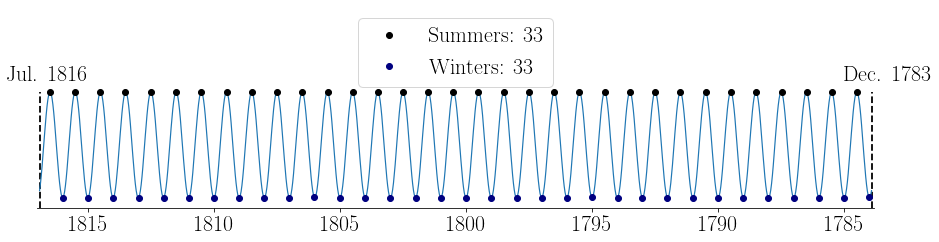
\includegraphics[width=\textwidth]{summersWinters_LT.png}
		\caption[Summers and Winters between Laki and Tambora]{Theoretical summers and winters in the time span between the Laki and Tambora volcanic depositions in Greenland.}
	\end{figure}
	
	Some measured signals in the ice cores contain annual cycles. For example, the water isotopes in the firn are sensitive to temperature, leading to a clear summer-to-winter cycle. This makes it relatively easy to date shallow ice cores as the cycles can be counted, but as diffusion takes place in the firn column, some of this signal is washed away. Luckily, another method can be utilized to date the ice: detection of known volcanic events through electrical conductivity measurements. By knowing the time of a certain volcanic event and matching this with the depth of the detected event in the ice, it is possible to set some very certain dates on the timescale of the ice. 
	
	An example of this volcanic event dating is through the volcanic eruptions of the Icelandic volcano Laki in 1783 and the Indonesian Volcano of Tambora in 1815. Both eruptions are very well historically documented and are visible and detectable in a great number of ice cores. This does not only make it possible to generally date different ice cores, but it also allows for in depth analysis of the diffusion and densification processes in the ice. 
	
	By considering an isotopic depth series situated between two volcanic events, it is possible to back diffuse this series over the known time span in years - or even months - using the diffusion length as a tuning parameter. This is an optimal way to empirically estimate the diffusion length of a given depth interval which makes it possible to obtain a temperature reconstruction of this interval, as $\sigma$ is temperature sensitive.
	
	The goal is thus to reconstruct the lost signal by a back diffusion scheme, tuning $\sigma$ of the diffusion process, until the known actual number of winters/summers can be counted as peaks and valleys in the depth signal. Then the estimated optimal diffusion length can be used to make a temperature estimate of the given interval.
	The back diffusion method is built on both empirical models and signal analysis of the measured data.
	
	\begin{figure}[h]
		\begin{tikzpicture}[node distance=1.1cm, auto]
			\node(in1) [io, text width=2.5cm, align=center] {Depth series,\\ $d$};
			\node(in2) [io, text width=3cm,align=center, left of=in1, xshift=-3.5cm] {Core \\specifications};
			\node(in3) [io, right of=in1, text width=2cm,xshift=2.5cm] {Constraints\\for $d$};
			
			\node(pro1) [process, text width=3cm, align=center, below of=in1, yshift=-.5cm] {Signal analysis};
			\node(pro2) [process, text width=3cm, align=center, below of=in2, yshift=-.5cm] {Models};
			\node(pro2pro1) [process, text width=2cm, align=center, below of=pro2, xshift=-1.5cm, yshift=-.3cm, scale=0.9] {Density};
			\node(pro2pro2) [process, text width=2cm, align=center, below of=pro2, xshift=1.5cm, yshift=-.3cm, scale=0.9] {Diffusion};
			
			\node(goal1) [decision, text width=5cm, below of=in1, yshift=-4cm, xshift=0cm,] {SIGNAL RESTORATION\\AND ENHANCEMENT};
			
			\node(goal2) [io, text width=3cm, below of=goal1, yshift=-.5cm,] {Optimal $\sigma$ estimate};
			\node(goal3) [io, text width=3cm, below of=goal2, yshift=-.5cm] {Temperature estimate, $T$};
			
			\draw[arrow] (in2) -- (pro2);
			\draw[arrow] (in1) -- (pro1);
			\draw[arrow] (pro2) -- (pro2pro1);
			\draw[arrow] (pro2) -- (pro2pro2);
			\draw[arrow] (pro1) -- (goal1);
			\draw[arrow] (in3) |- (goal1);
			\draw[arrow] (pro2pro1) |- (goal1);
			\draw[arrow] (pro2pro2) |- (goal1);
			\draw[arrow] (goal1) -- (goal2);
			\draw[arrow] (goal2) -- (goal3);
			%		\node(empty1) [below of=in1, xshift=3.2cm] {Analysis};
			%		\node(pro1) [process, below of=empty1, yshift=-0.3cm, text width=4cm, align=center] {Find optimal $\sigma$ that fulfills constraints};
			%		\node(pro2) [process, below of=pro1, text width=4cm, yshift=-0.5cm, align=center] {Temperature estimate based on $\sigma_{\text{opt}}$};
			%		
			%		\draw[-] (in1) -| (empty1);
			%		\draw[-] (in2) -| (empty1);
			%		\draw[arrow] (empty1) -- (pro1);
			%		\draw[arrow] (pro1) -- (pro2);
		\end{tikzpicture}
		\caption{For Introduction}
	\end{figure}
	
	
	\section[Using the Rare Gem]{Utilizing the Rare Gem}
	\label{Sec:UtilizinGem}
	In this thesis an introduction to diffusion of water isotopes in ice cores is firstly presented along with methods for modeling densification and diffusion profiles. Following is a brief examination of different experimental methods for detection of volcanic deposited material and which methods has been used for the data under inspection. The chosen data are then presented along with an argumentation of why they were selected. Then a thorough presentation of data and signal analysis along with important computational methods are presented. These different tools are then combined in the method description, depicting a walk-through and testing of the final algorithm developed for estimating the diffusion length given the specific number of years. The final method is tested and further developed and fine tuned, and results given the last iteration of the method are presented. On the basis of these results, finally, a temperature reconstruction of the area of the drill sites is attempted. 
	
	
%	\section{Old}
%	
%	Many analyses of ice cores have mainly focused on the large scale changes happening over hundreds, thousands and tens of thousands of years, [\ref{label}] \todo{INTRO: REFERENCES and examples}.	When considering such large-scale changes, it is acceptable that the dating of the ice core is off by a year or two as the interest is mainly on the general trends over many years and not on individual annual changes. This is rather lucky, as it is rare to have exact and precise dating, especially in older and deeper cores where the annual layer cycles have been extinguished. 
%	
%	
%	The scope of this project though, has a different focus: When examining ice core data for volcanic eruptions through, for example, electrical conductivity measurements, it is sometimes possible to date the ice cores much more accurate and precise. Two aspects are in play here: Firstly, if volcanic eruptions are visible in more than one ice core it is possible to synchronize all measured quantities in these cores by matching their volcanic profiles. This enhances the accuracy of the dating and also presents the possibility to examine more local behaviors of the Earth system as, for example, cross-hemisphere data can be compared. Secondly, if the eruptions have been recorded in human history, the precision of the dating can be highly improved, as these historical records often contain both time, place, duration and other important parameters of the volcanic events. For this project both aspects are considered as the focus is on the volcanic eruptions of the Icelandic volcano Laki in 1783 and the Indonesian volcano Tambora in 1815, which are both very well historically recorded and documented and are both visible in a great number of ice cores. 
%	
%	This reveals a rare gem of knowledge: as the two eruptions are relatively close in time, well documented and detectable in many cores, it is possible to say with high confidence that any data measured and analyzed, be it isotopic, conductivity, chemical ot otherwise, in the ice core section between these two visible eruptions, must in time represent the time span between the deposition of volcanic material at the ice core site. This allows for in depth analysis of the diffusion and densification processes the ice has been through and makes it possible to examine and develop new methods to restore diffused signals and otherwise lost information with high precision and accuracy. This is mainly due to the constraints raised based on the knowledge of deposition time: Since there are 33 years between the volcanic depositions, there must be detected exactly 33 winters and 33 summers in the isotopic signals. Thus, the restoration of the diffused data series can be optimized to fulfill these criteria.
%	
%	All of this presents a way to make more precise local temperature estimates over a shorter time period through the different temperature proxies present in the ice core data.
	%\section[Laki and Tambora]{Laki and Tambora in Recorded History}
	%In the not-so-distant past two volcanic horizons have been of great importance for this thesis, namely the Laki eruption in 1783 and the Tambora eruption of 1815. Interestingly, these eruptions have not only impacted the geophysical world, but has left their footprints on the history of Man in politics[REFERENCE], sociology[REFERENCE], arts[REFERENCE] and philosophy[REFERENCE]. On the eighth day of June in 1783 a volcanic fissure located in the southern part of Iceland was central for a global climatic change. The fissure Lakagígar or more commonly known as Laki refering to the central mountain, erupted with violent phreagomagmatic explosions due to the basalt magma being exposed to ground water. The eruption was given a Volcanic Explosivity Index(VEI) of 4, corresponding to the magnitude of the much later 2010 Eyjafjallajökull Icelandic eruption. For the next eight months the fissure continued to emit great amounts of sulfuric aerosols into the atmosphere, resulting locally in Iceland in catastrophic mass famine, due to loss of livestock to poisoning, with up to 25 \% of the population dying from starvation and poisoning from the volcanic gasses. Globally, the eruption caused a huge amount of sulfur dioxide to be spewed into the northern hemisphere which led to a global drop in temperatures and a generally more extreme climate. In the European regions the following summer was much warmer than usual with many thunderstorms to follow. The winter of 1783-84 was subsequently extreme, with long periods of continuous frost. In France the late 1780's were marked by several years with droughts in the summer and frost in the winter, which contributed greatly to a rise in poverty and famine, and creating a greater division between the people and the rulers. Along with a growing dismay and distrust in the ruling forces the climatic changes due to Laki and a number of other climatic disruptions the French political situation finally climaxed in the French revolution of 1789. [REFERENCES!!!!]\\
	%32 years later on April 5 in 1815 an even more powerful eruption ensued: the eruption of Mount Tambora on the, now, Indonesian island Sumbawa. This eruption had a Volcanic Explosivity Index of 7, which makes it the most powerful in the recorded history of humankind. Considering that the VEI is defined as a logarithmic scale - at least for indices larger than VEI-3 - the Tambora eruption, though located just south of the Equator, impacted the entire globe as well as the European continent in at least the same magnitude as the 32 years prior Laki eruption. Locally, it was estimated to cause at least 10,000 direct deaths and many tens of thousands more due to sulfur dioxid poisoning, famine and disease. In many contexts the year of 1816 following the event became known as "\textit{The Year Without a Summer}", as the ashes from the eruption column dispersed across the world and lowered global temperatures. This significant climate change though was not just a consequence of the Tambora eruption, but was pushed by a number of climatic forcings, some due to several previous volcanic activities around the globe. Combined, these effects coincided in a drop in global temperature by about 0.4 to 0.7 $^{\circ}$C. This climatic change affected the entire globe by disrupting the Indian monsoons, causing a number of failed harvests, laying ground to severe typhus epidemics in southeast Europe and destroying crops and causing potato, oat and what harvest failure, especially in Ireland. Since the eruption had so severe consequences for the day to day lives of many people, the aftermath all around the world has been one of the greatest documented in recorded time, with a clear impact on the works of many artists, among them Lord Byron and J. M. W Turner[REFERENCES!!!!]. Although both eruptions caused many a tragedy, there is beauty in using these events as volcanic horizons in ice core records. Given the severity of both eruptions, they have been so well documented in historical records that they make up solid and certain pillars in developing a temporal map of the past life of our ever so active earth. For that and for their brutal beauty they will remain in human history for a great while to come.
	
\end{document}